\documentclass[journal,12pt,onecolumn]{IEEEtran}
\usepackage[utf8]{inputenc}   % Codificación de entrada
\usepackage[T1]{fontenc}      % Codificación de fuente
\usepackage[spanish,es-tabla]{babel}   % Idioma español
\usepackage{lmodern}          % Fuente moderna
\usepackage{amsmath, amssymb} % Matemáticas y símbolos
\usepackage{graphicx} 		  % Gráficos e imágenes
\graphicspath{{img/}{tablas/}{portada/}}  % Las imágenes se buscarán en la carpeta "img"
\usepackage{longtable}      % Para tablas que se extienden en varias páginas
\usepackage{tabularx}	% Tablas avanzadas
\usepackage{threeparttable}
\usepackage{hyperref}	% Hipervínculos
\usepackage{float} % va a servir para los espacios entre fotos supuestamente


%-------------------------------------------
% Otros paquetes útiles (personaliza según tus necesidades)
%-------------------------------------------
\usepackage{caption}
\usepackage{subcaption}
\usepackage{xcolor}
\usepackage{setspace}

%-------------------------------------------
% Comandos personalizados
\renewcommand{\listtablename}{Índice de tablas}
\renewcommand{\appendixname}{Anexos}
\definecolor{colorreferences}{RGB}{48,134,3}

% Metadatos del PDF
\hypersetup{
	unicode=true,
	hidelinks,
	colorlinks=true,       % false: boxed links; true: colored links
	linkcolor=black,          % color of internal links (change box color with linkbordercolor)
	citecolor=colorreferences,        % color of links to bibliography
	filecolor=magenta,      % color of file links
	urlcolor=blue,           % color of external links
	linkbordercolor={0 0 0}
}
%-------------------------------------------
% Inicio del documento
%-------------------------------------------
\begin{document}

% Aquí se encuentra el archivo con la portada
\begin{titlepage}
	\centering
	%-------------------------------------------
	% Logos en una tabla: izquierda, centro y derecha
	\begin{tabular}{@{}p{0.3\textwidth} p{0.3\textwidth} p{0.3\textwidth}@{}}
		
\includegraphics[height=2cm]{tecnm} & 
		\centering 
\includegraphics[height=1.5cm]{SEP} & 
		\raggedleft 
\includegraphics[height=2cm]{ith.jpg} \\
	\end{tabular}
	
	\vspace{2em}
	
	\noindent
	%-------------------------------------------
	%	Información institucional y académica (esquina superior izquierda)
	\begin{minipage}[t]{0.48\textwidth}
		\raggedright
		\small \textbf{%
			Instituto Tecnológico de Hermosillo\\
			Materia: Robótica\\
			Profesor: Medina Gil Lamadrid, Jesús Iván%
		}
	\end{minipage}%
	\hfill
	%	fecha actual (esquina superior derecha), en letras pequeñas y en negrita.
	\begin{minipage}[t]{0.48\textwidth}
		\raggedleft
		\small \textbf{\today}
	\end{minipage}
	
	\vspace{2em}
	
	%-----------------------------------------
	% Unidad y Título de la tarea en letras grandes y en negrita
	{\large \textbf{Unidad 1: Morfología del robot}}\\
	{\Huge \textbf{Tipos de Sensores}}
		
	\vspace{1em}
	
	%---------------------------------------
	% Tabla con la información del equipo
	%---------------------------------------
	% Encabezado del equipo
	\begin{center}
		{\Large \textbf{Equipo 2}}
	\end{center}
	
	\vspace{1em}
	
	% Tabla de integrantes:
	% Cada fila contiene: foto (columna izquierda) y datos del integrante (columna derecha)
	\begin{center}
		\begin{tabular}{c c}
			\begin{tabular}{c}
				
\includegraphics[height=3cm]{Cedano.jpeg} \\
				\textbf{Cedano Mendoza},\\ Carlos Francisco \\ \texttt{L21330552@hermosillo.tecnm.mx} \\ Teléfono: 6624686707
			\end{tabular} &
			\begin{tabular}{c}
				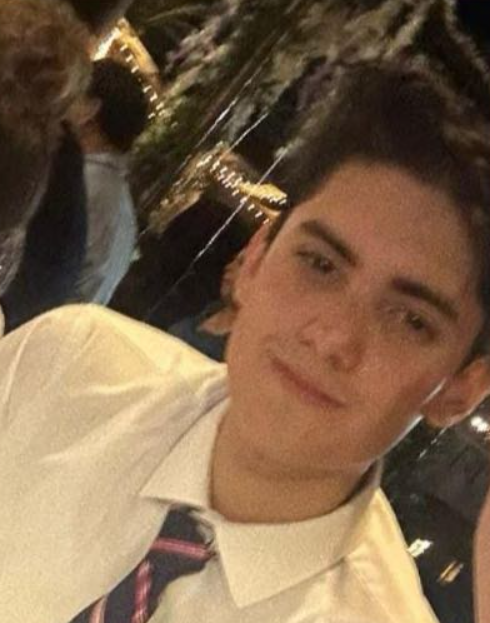
\includegraphics[height=3cm]{Martinez.png} \\
				\textbf{Martinez Navarro,}\\ Sebastian \\ \texttt{L2133} \\ Teléfono: 6621053764
			\end{tabular} \\ \vspace{2em}
			\begin{tabular}{c}
				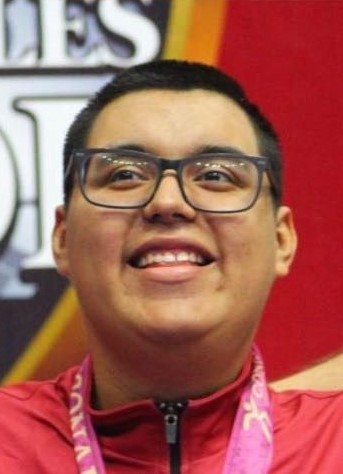
\includegraphics[height=3cm]{Ocampo.jpeg} \\
				\textbf{Ocampo Ramos,}\\ Addiel Adrián \\ \texttt{L20330895@hermosillo.tecnm.mx} \\ Teléfono: 6623501716
			\end{tabular} &
			\begin{tabular}{c}
				\includegraphics[height=3cm]{Pérez.jpeg} \\
				\textbf{Pérez Estupiñán,}\\ Ana Claudia \\ \texttt{L21330669@hermosillo.tecnm.mx} \\ Teléfono: 6624281154
			\end{tabular}
		\end{tabular}
	\end{center}

\end{titlepage}

%	Es innecesario poner el índice porque ya aparece en los marcadores del PDF
%\tableofcontents

% Ejemplo de inclusión de una sección (por ejemplo, "introduccion.tex" debe estar en la carpeta "secciones" y se recomienda no usar carácteres especiales (tilde) o espacios)


 \section{Cinemática Inversa}


	\subsection{Robot 6}
	   \begin{figure}[H]
	   	\centering
	   	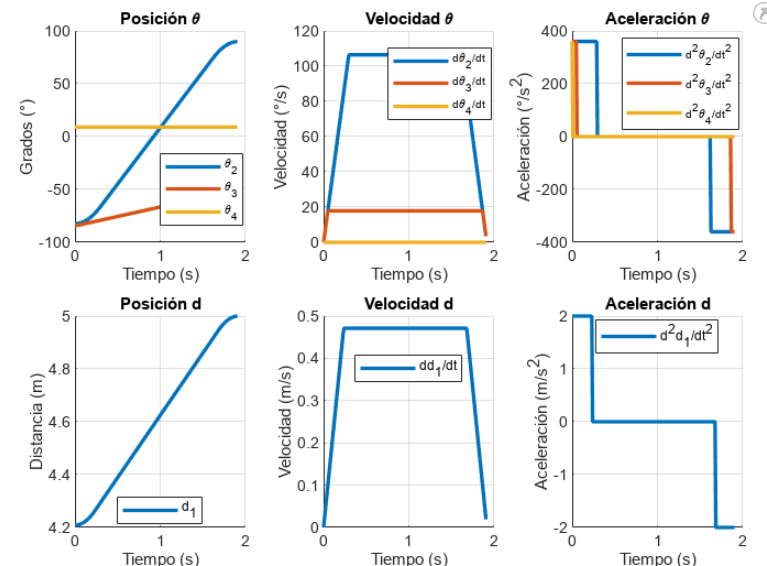
\includegraphics[width=0.8\textwidth]{R6_cinematica_articular}
	   	\caption{Cinemática articular del robot 6: posición, velocidad y aceleración de las articulaciones en función del tiempo.}
	   	\label{fig:cinematica_articular}
	   \end{figure}
	   
	   \begin{figure}[H]
	   	\centering
	   	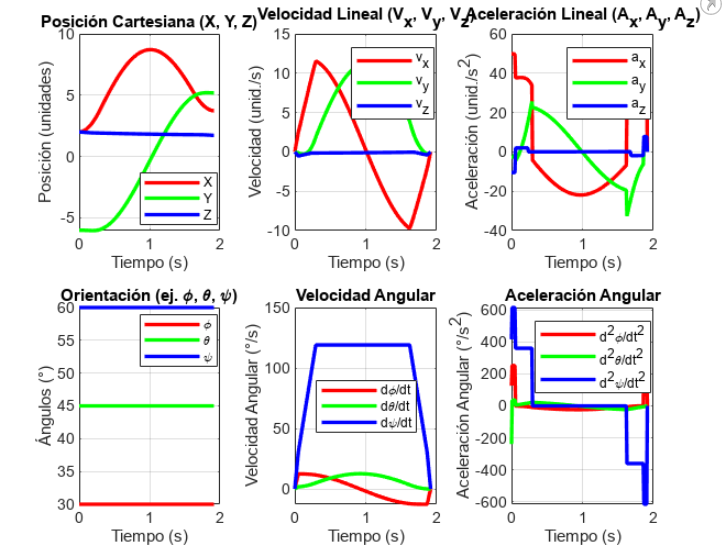
\includegraphics[width=0.8\textwidth]{R6_graficas_1}
	   	\caption{Cinemática cartesiana del robot 6: posición, velocidad y aceleración lineal y angular en función del tiempo.}
	   	\label{fig:cinematica_cartesiana}
	   \end{figure}
	   
	   \begin{figure}[H]
	   	\centering
	   	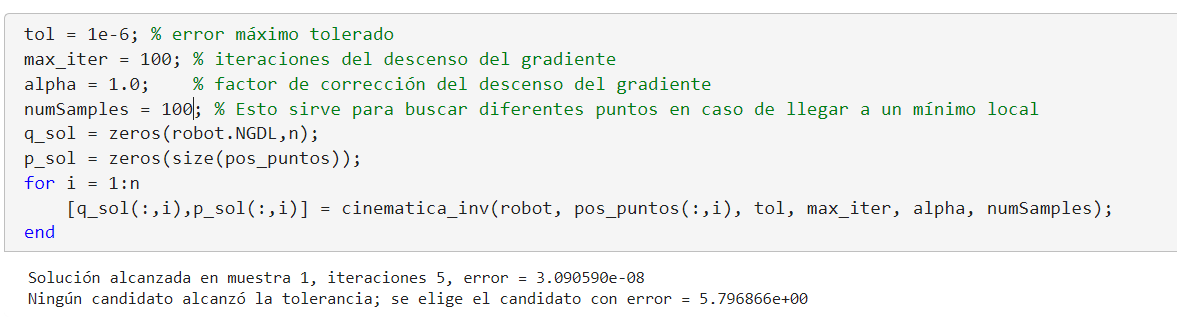
\includegraphics[width=1\textwidth]{R6_error}
	   	\caption{Error del objetivo del robot 6.}
	   	\label{fig:error_objetivo6}
	   \end{figure}
	   
			
			
	\subsection{Robot 7}
	\begin{figure}[H]
		\centering
		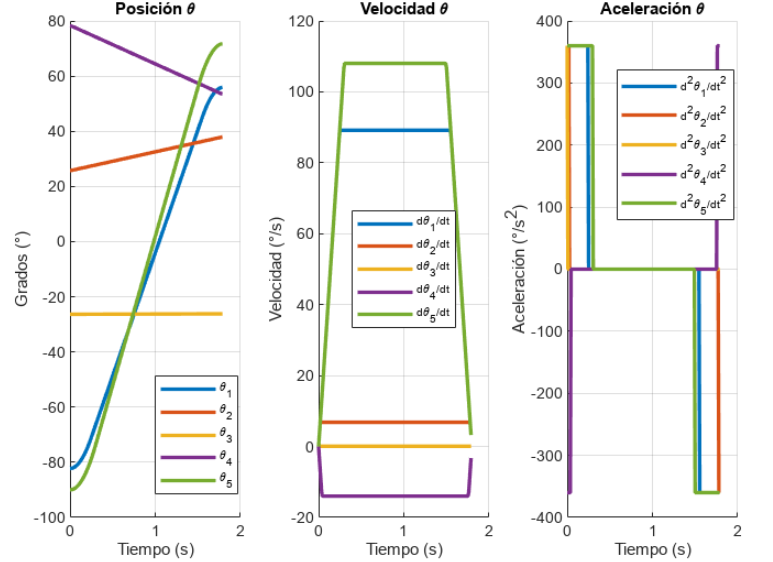
\includegraphics[width=0.65\textwidth]{R7_cinematica_art}
		\caption{Cinemática articular del robot 7: posición, velocidad y aceleración de las articulaciones en función del tiempo.}
		\label{fig:R7_cinematica_articular}
	\end{figure}
	
	\begin{figure}[H]
		\centering
		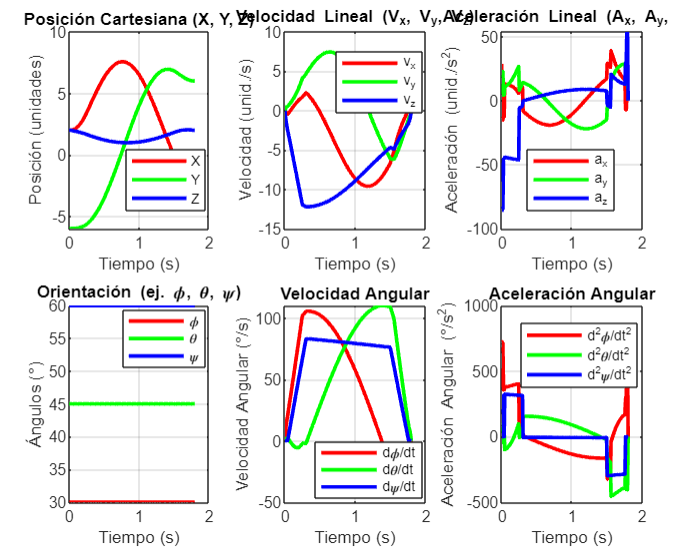
\includegraphics[width=0.65\textwidth]{R7_graficas}
		\caption{Cinemática cartesiana del robot R7: posición, velocidad y aceleración lineal y angular en función del tiempo.}
		\label{fig:R7_cinematica_cartesiana}
	\end{figure}
	
	\begin{figure}[H]
		\centering
		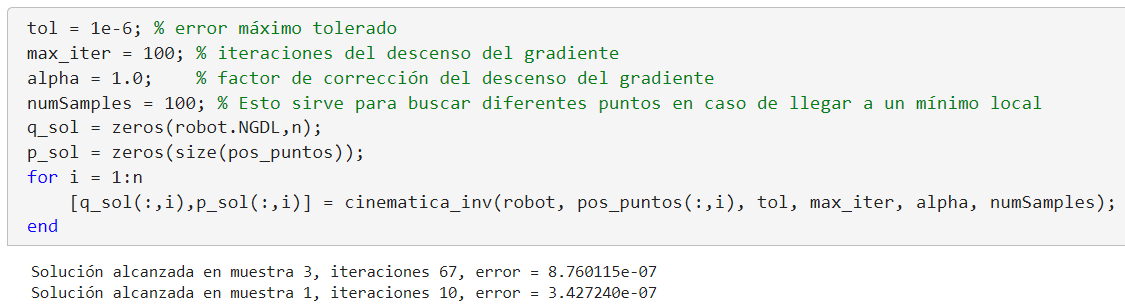
\includegraphics[width=1\textwidth]{R7_error}
		\caption{Error del objetivo del robot 7.}
		\label{fig:R7_error_objetivo7}
	\end{figure}
	
	

\section{Conclusión}
En la elaboración de este reporte, se utilizó por primera vez el software LaTeX para la edición del documento y Sourcetree para la gestión del control de movimientos entre modificaciones de datos del documento por parte de los distintos miembros del equipo. A lo largo del proceso, se presentaron dificultades relacionadas con el uso de Sourcetree, especialmente en la ejecución de comandos como branches, commit, push y pull, lo que requirió una curva de aprendizaje adicional para comprender su funcionamiento y evitar conflictos en la sincronización de archivos.

A pesar de estos desafíos, la experiencia permitió familiarizarse con herramientas clave para la edición y gestión colaborativa de documentos, lo que resultará beneficioso en futuros proyectos. La combinación de LaTeX y Sourcetree demostró ser una opción robusta para la elaboración de reportes técnicos con un control de organización eficiente, aunque es recomendable seguir profundizando en su uso para optimizar los flujos de trabajo y minimizar errores.

Por otra parte, el conocimiento más importante obtenido de la investigación sobre los distintos tipos de sensores fue la comprensión de cómo cada tecnología responde a necesidades específicas en diversas industrias. Esta investigación permitió no solo identificar las aplicaciones clave de cada sensor, sino también comprender la importancia de la selección adecuada según el entorno y el tipo de medición requerida. La evolución de los sensores, junto con su integración con inteligencia artificial y procesamiento de datos, sigue impulsando innovaciones en automatización, control y análisis del entorno.








	
\end{document}
